\documentclass[11pt,oneside,letterpaper]{article}

% graphicx package, useful for including eps and pdf graphics
\usepackage{graphicx}
\DeclareGraphicsExtensions{.pdf,.png,.jpg}

% basic packages
\usepackage{color} 
\usepackage{parskip}
\usepackage{float}

% text layout
\usepackage{geometry}
\geometry{textwidth=15cm} % 15.25cm for single-space, 16.25cm for double-space
\geometry{textheight=22cm} % 22cm for single-space, 22.5cm for double-space

% helps to keep figures from being orphaned on a page by themselves
\renewcommand{\topfraction}{0.85}
\renewcommand{\textfraction}{0.1}

% bold the 'Figure #' in the caption and separate it with a period
% Captions will be left justified
\usepackage[labelfont=bf,labelsep=period,font=small]{caption}

% review layout with double-spacing
%\usepackage{setspace} 
%\doublespacing
%\captionsetup{labelfont=bf,labelsep=period,font=doublespacing}

% cite package, to clean up citations in the main text. Do not remove.
\usepackage{cite}
\usepackage{hyperref}
%\renewcommand\citeleft{(}
%\renewcommand\citeright{)}
%\renewcommand\citeform[1]{\textsl{#1}}

% Remove brackets from numbering in list of References
\renewcommand\refname{\large References}
\makeatletter
\renewcommand{\@biblabel}[1]{\quad#1.}
\makeatother

\usepackage{authblk}
\renewcommand\Authands{ \& }
\renewcommand\Authfont{\normalsize \bf}
\renewcommand\Affilfont{\small \normalfont}
\makeatletter
\renewcommand\AB@affilsepx{, \protect\Affilfont}
\makeatother

% comments
\usepackage{ulem}
\definecolor{purple}{rgb}{0.459,0.109,0.538}
\def\tb#1#2{\sout{#1} \textcolor{purple}{#2}} 
\def\tbc#1{\textcolor{purple}{[#1]}}

\title{\vspace{1.0cm} \LARGE \bf Phylogenetic analysis of Guinea 2014 EBOV ebolavirus outbreak}

\author[1]{Gytis Dudas}
\author[1,2,3]{Andrew Rambaut}

\affil[1]{Institute of Evolutionary Biology, University of Edinburgh, Edinburgh, UK}
\affil[2]{Fogarty International Center, National Institutes of Health, Bethesda, MD, USA}
\affil[3]{Centre for Immunology, Infection and Evolution at the University of Edinburgh, Edinburgh, UK}

\begin{document}
\maketitle

\section*{Introduction}
%\begin{abstract}
A recent article \cite{baize2014} suggests that the currently ongoing outbreak in Guinea is caused by a divergent variant of the Zaire ebola (EBOV) lineage. The EBOV strain has previously caused ebola outbreaks in the Democratic Republic of Congo (DRC) and Gabon. The authors publish three complete genome sequences from the Guinea outbreak and perform a phylogenetic analysis using 24 sequences of Zaire and other representative lineages. One finding of this is that the 2014 sequences fall as a divergent lineage outside the Zaire lineage suggesting that this may be a pre-existing endemic virus in West Africa rather than the result of spread of the EBOV lineage from the Central African countries that have had previous human outbreaks.
%\end{abstract}

\section*{Materials and methods}
All complete genome sequences from the genus Ebolavirus (which includes Bundibugyo BDBV, Reston RESTV, Sudan SUDV, Tai Forest TAFV and Zaire ebolavirus EBOV species) were collated from genbank including the sequences from the Guinea outbreak.
Genbank accessions and sources for the sequences can be found at \url{http://epidemic.bio.ed.ac.uk/ebolavirus_sequences} .
We would like to thank Stephan G\"{u}nther and his co-authors for sending us the sequences from the Guinea outbreak. 

We extracted the coding sequences of each gene. 
The Ebolavirus genome consists of a single strand of negative sense single stranded RNA and contains 7 protein coding genes (in order 3'-NP-VP35-VP40-GP-VP30-VP24-L, separated by various intergenic regions) \cite{sanchez1993}.
Two alignments were concatenated derived from coding and non-coding regions of the genomes.
Trees were analyzed in PhyML \cite{guindon2003} or MrBayes \cite{huelsenbeck2001} using GTR (\tbc{?}) \cite{miura1986} substitution model.

When analyzed in BEAST \cite{drummond2012} the complete genome sequences gave inconsistent results and BEAST appeared to be sampling from a bimodal posterior distribution.
We thus compiled a dataset containing only the glycoprotein (GP) sequences, for which more sequences are available.
Many of the extra sequences came from wild ape carcasses \cite{wittmann2007} in Gabon and DRC.
These sequences were analyzed in BEAST \cite{drummond2012} to find out when the lineage that caused the outbreak in Guinea split from other EBOV lineages.
The data were analyzed using a GTR+$\Gamma$ nucleotide substitution model, and either an uncorrelated relaxed (following a lognormal distribution) \cite{drummond2006} or a strict molecular clock and under different demographic models (constant population size, exponential growth or the non-parametric Bayesian skyride \cite{minin2008}).
This dataset was found to be quite robust to different demographic models, but more uncertainty in inferred node dates was noticed when using a strict molecular clock.
We use the results from a relaxed molecular clock analysis, under an exponential growth tree prior (as it can accomodate a constant population size scenario when the growth rate is 0).

\section*{Analysis}
An alignment of complete genomes and a maximum likelihood tree (PhyML) confirms the phylogenetic position shown in the recent paper \cite{baize2014} (Figure \ref{NEJMtree}).
\begin{figure}[h!]
\centering  
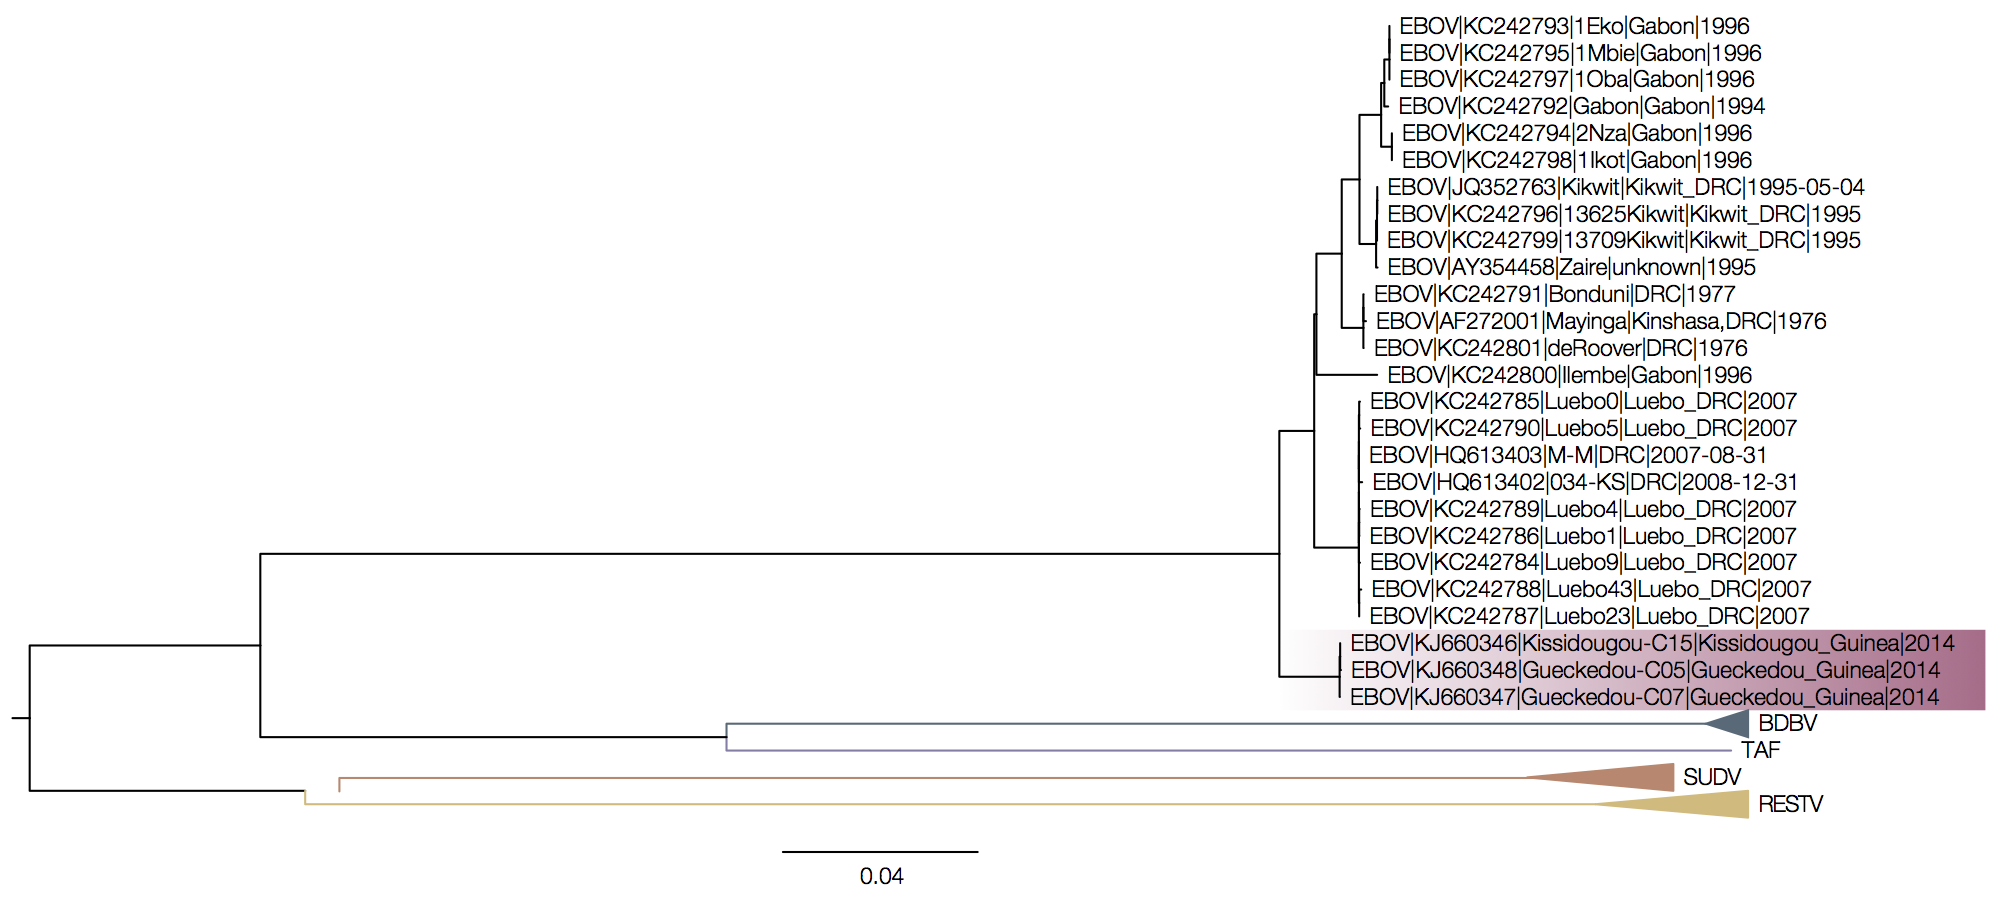
\includegraphics[width=1\textwidth]  {figures/ebolavirus_raw_ml_tree.png}
\caption{\textbf{ML tree of complete genomes.}
Replicated analysis from Baize \textit{et al}. \cite{baize2014} identifies the Guinea outbreak sequences (highlighted) as belonging to a divergent EBOV lineage.
Tips belonging to EBOV lineage are not collapsed.}
\label{NEJMtree}
\end{figure}

When the intergenic sequences are removed, however, the Guinea outbreak sequences fall within the diversity of Zaire ebolavirus (Figure \ref{MBtreeCDS}).
We suspect the discrepancy between our results and those of Baize \textit{et al}. \cite{baize2014} arose through long branch attraction.
EBOV lineages are rather poorly sampled and sequences from most outbreaks, because of the nature of the outbreaks, have nearly identical sequences.

\begin{figure}[h!]
\centering  
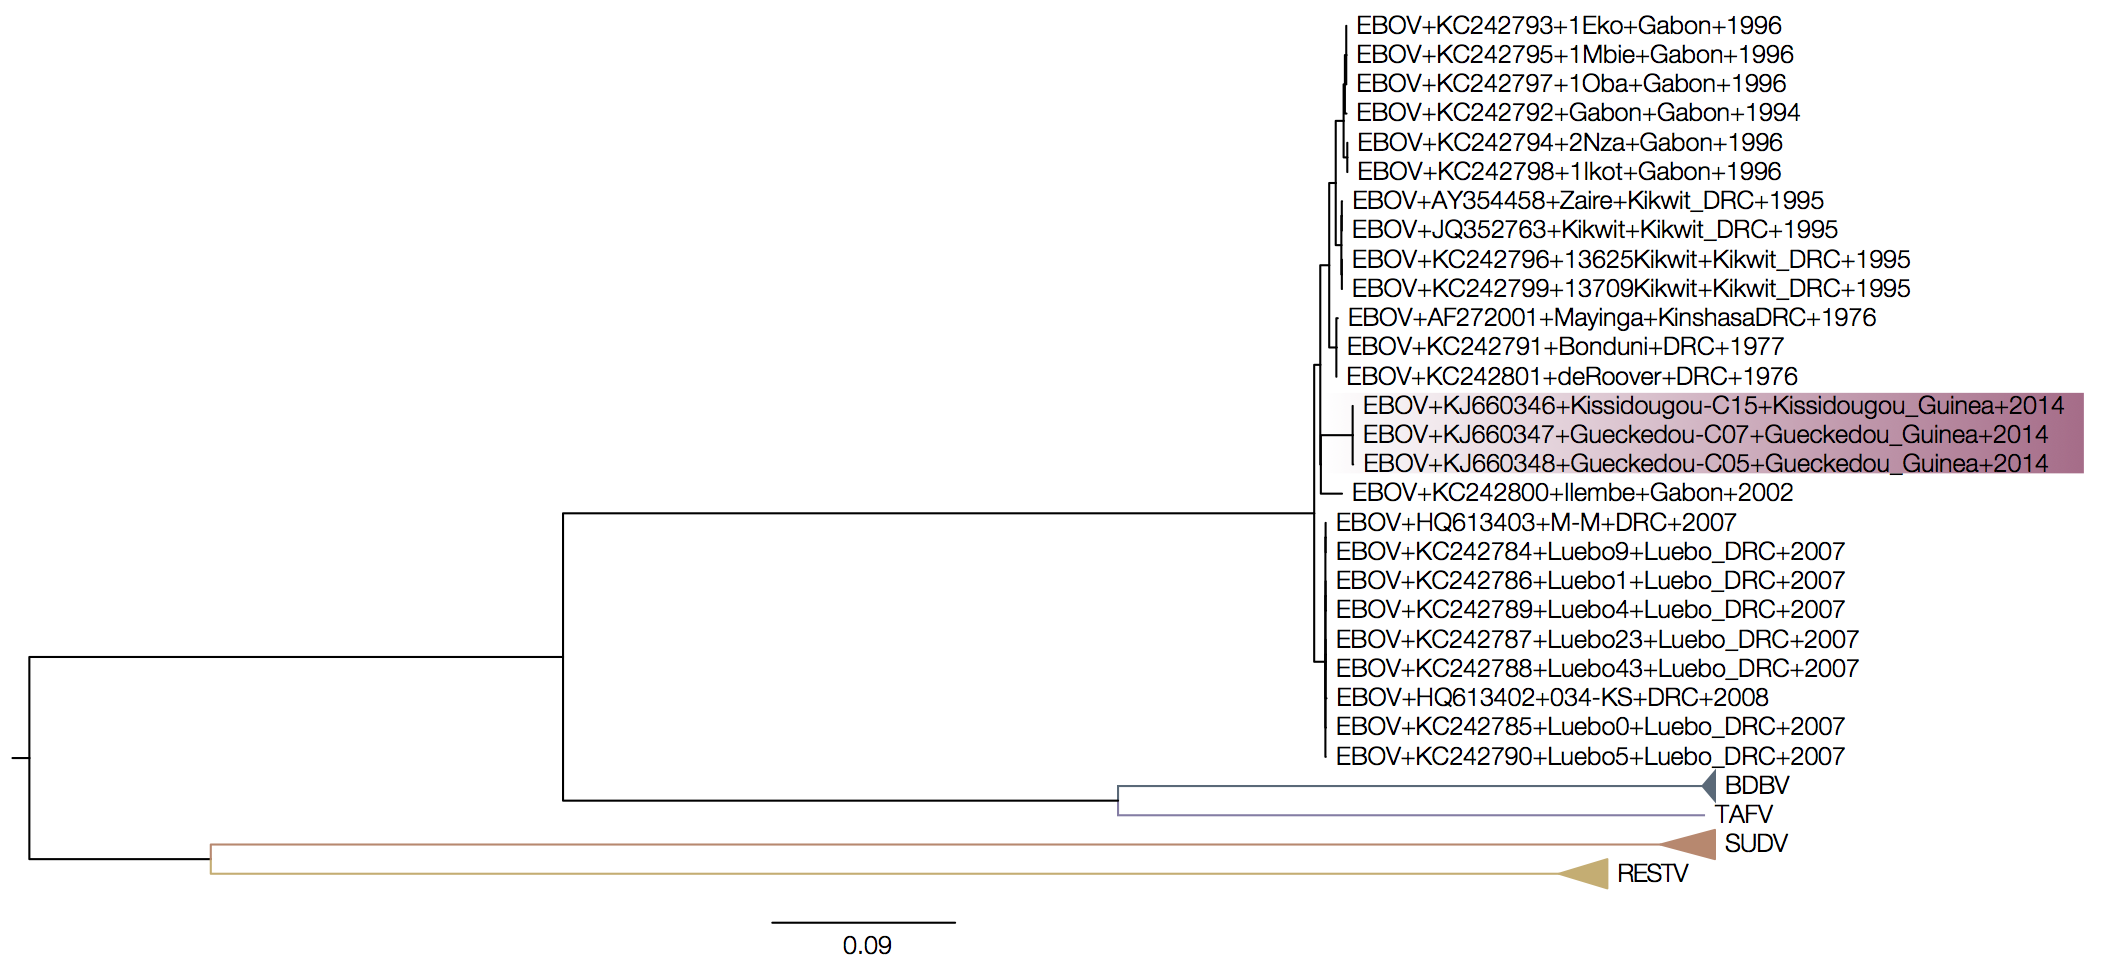
\includegraphics[width=1\textwidth]  {figures/ebolavirus_cds_mb_tree.png}
\caption{\textbf{MrBayes tree of concatenated coding sequences.}
When only the coding sequences are used, the Guinea outbreak sequences appear to be derived from within the diversity of Gabon/DRC EBOV lineages.}
\label{MBtreeCDS}
\end{figure}

\begin{figure}[h!]
\centering  
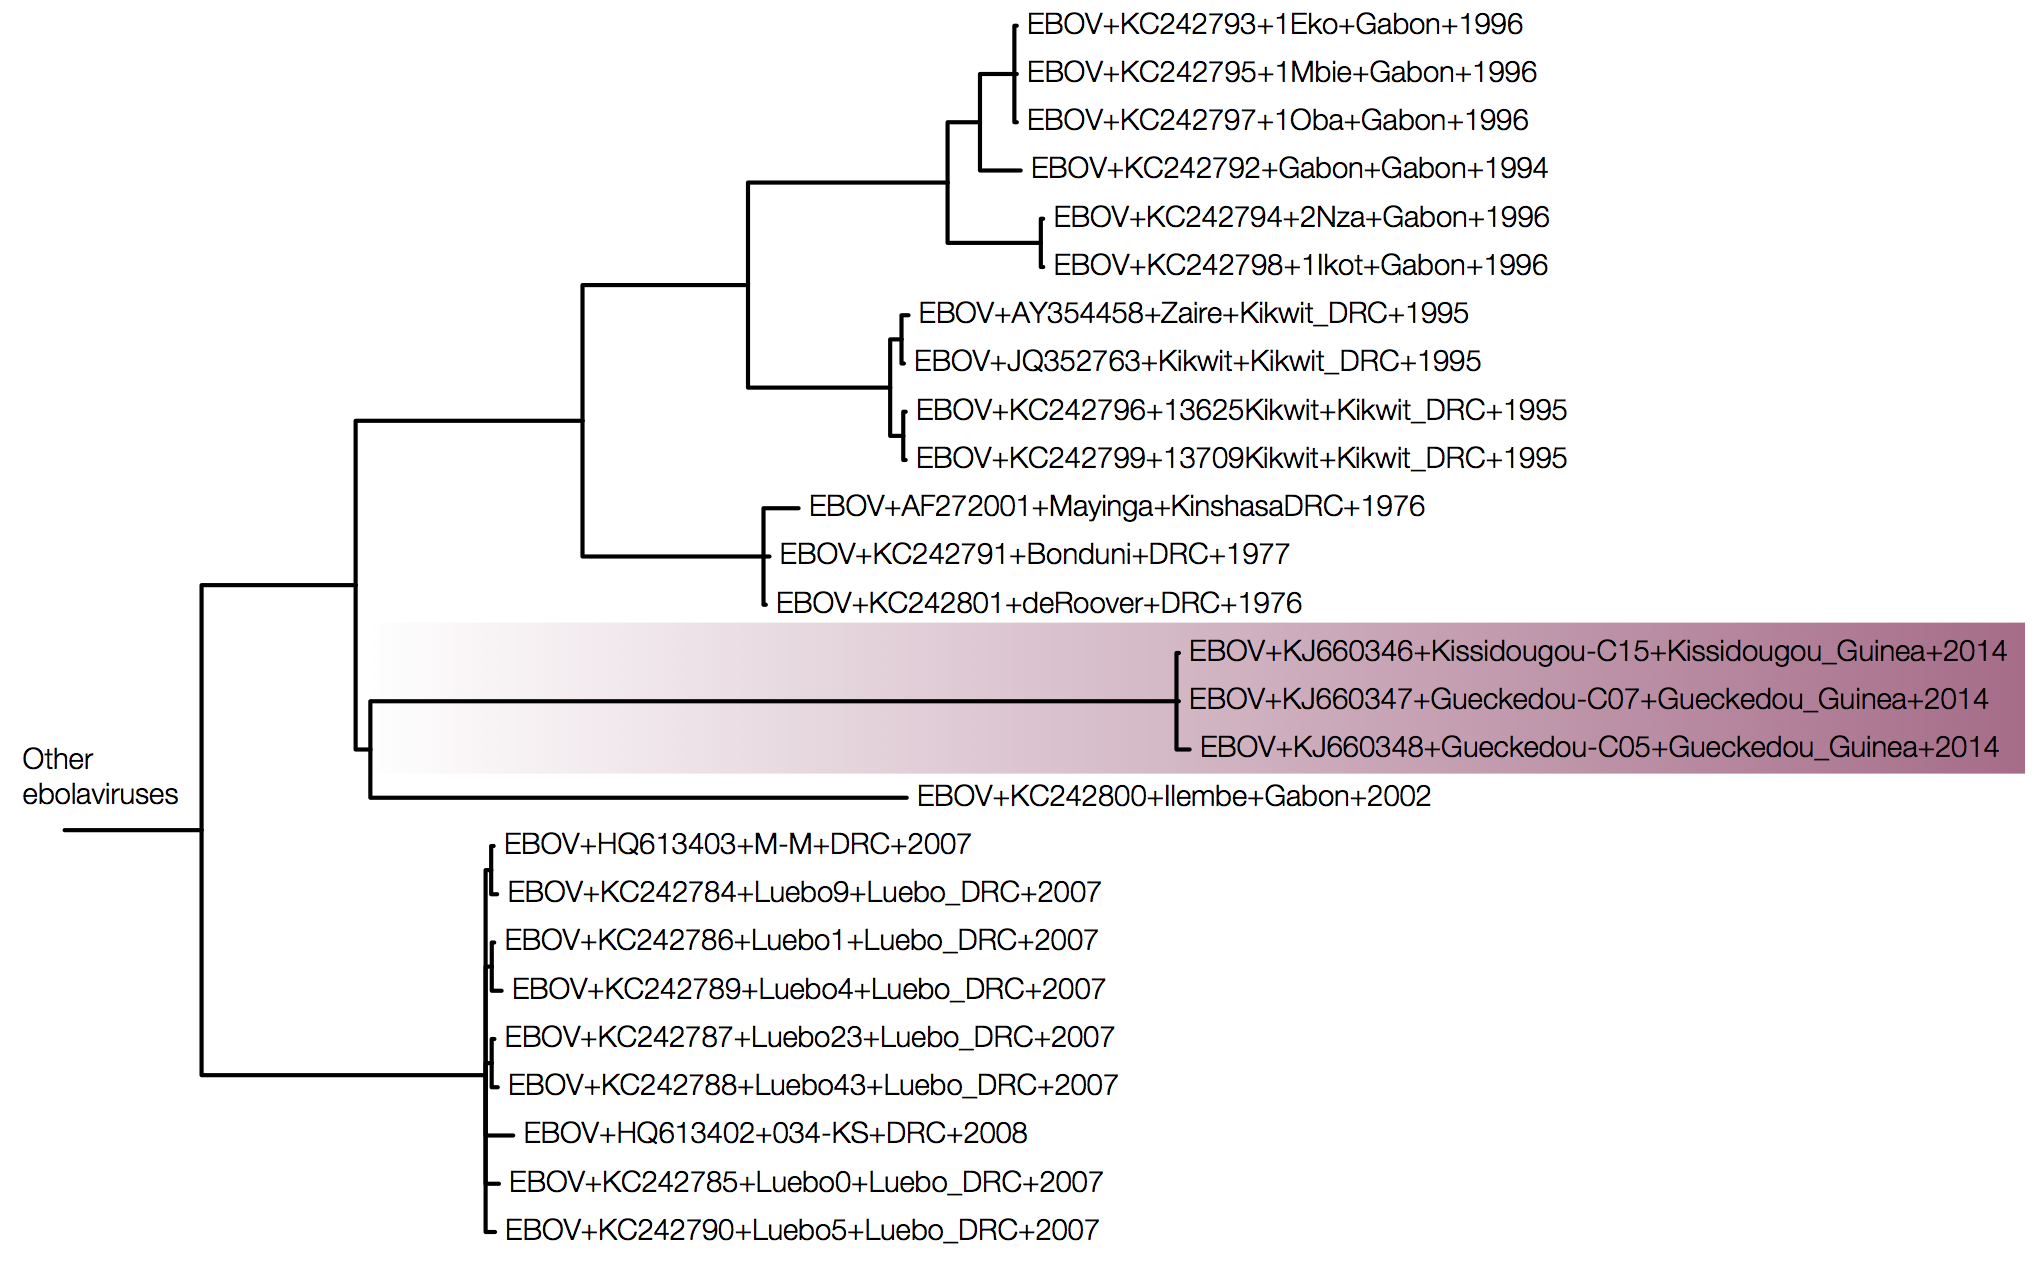
\includegraphics[width=1\textwidth]  {figures/EBOV_cds_mb_tree.png}
\caption{\textbf{Expanded view of a MrBayes tree of concatenated coding sequences.}
Expanding the EBOV region of the tree (same tree as Figure \ref{MBtreeCDS}, but with the divergent ebolavirus species cropped out) we see that the Guinea outbreak sequences are nested within the EBOV clade.}
\label{MBtreeCDSzoomed}
\end{figure}

\begin{figure}[h!]
\centering  
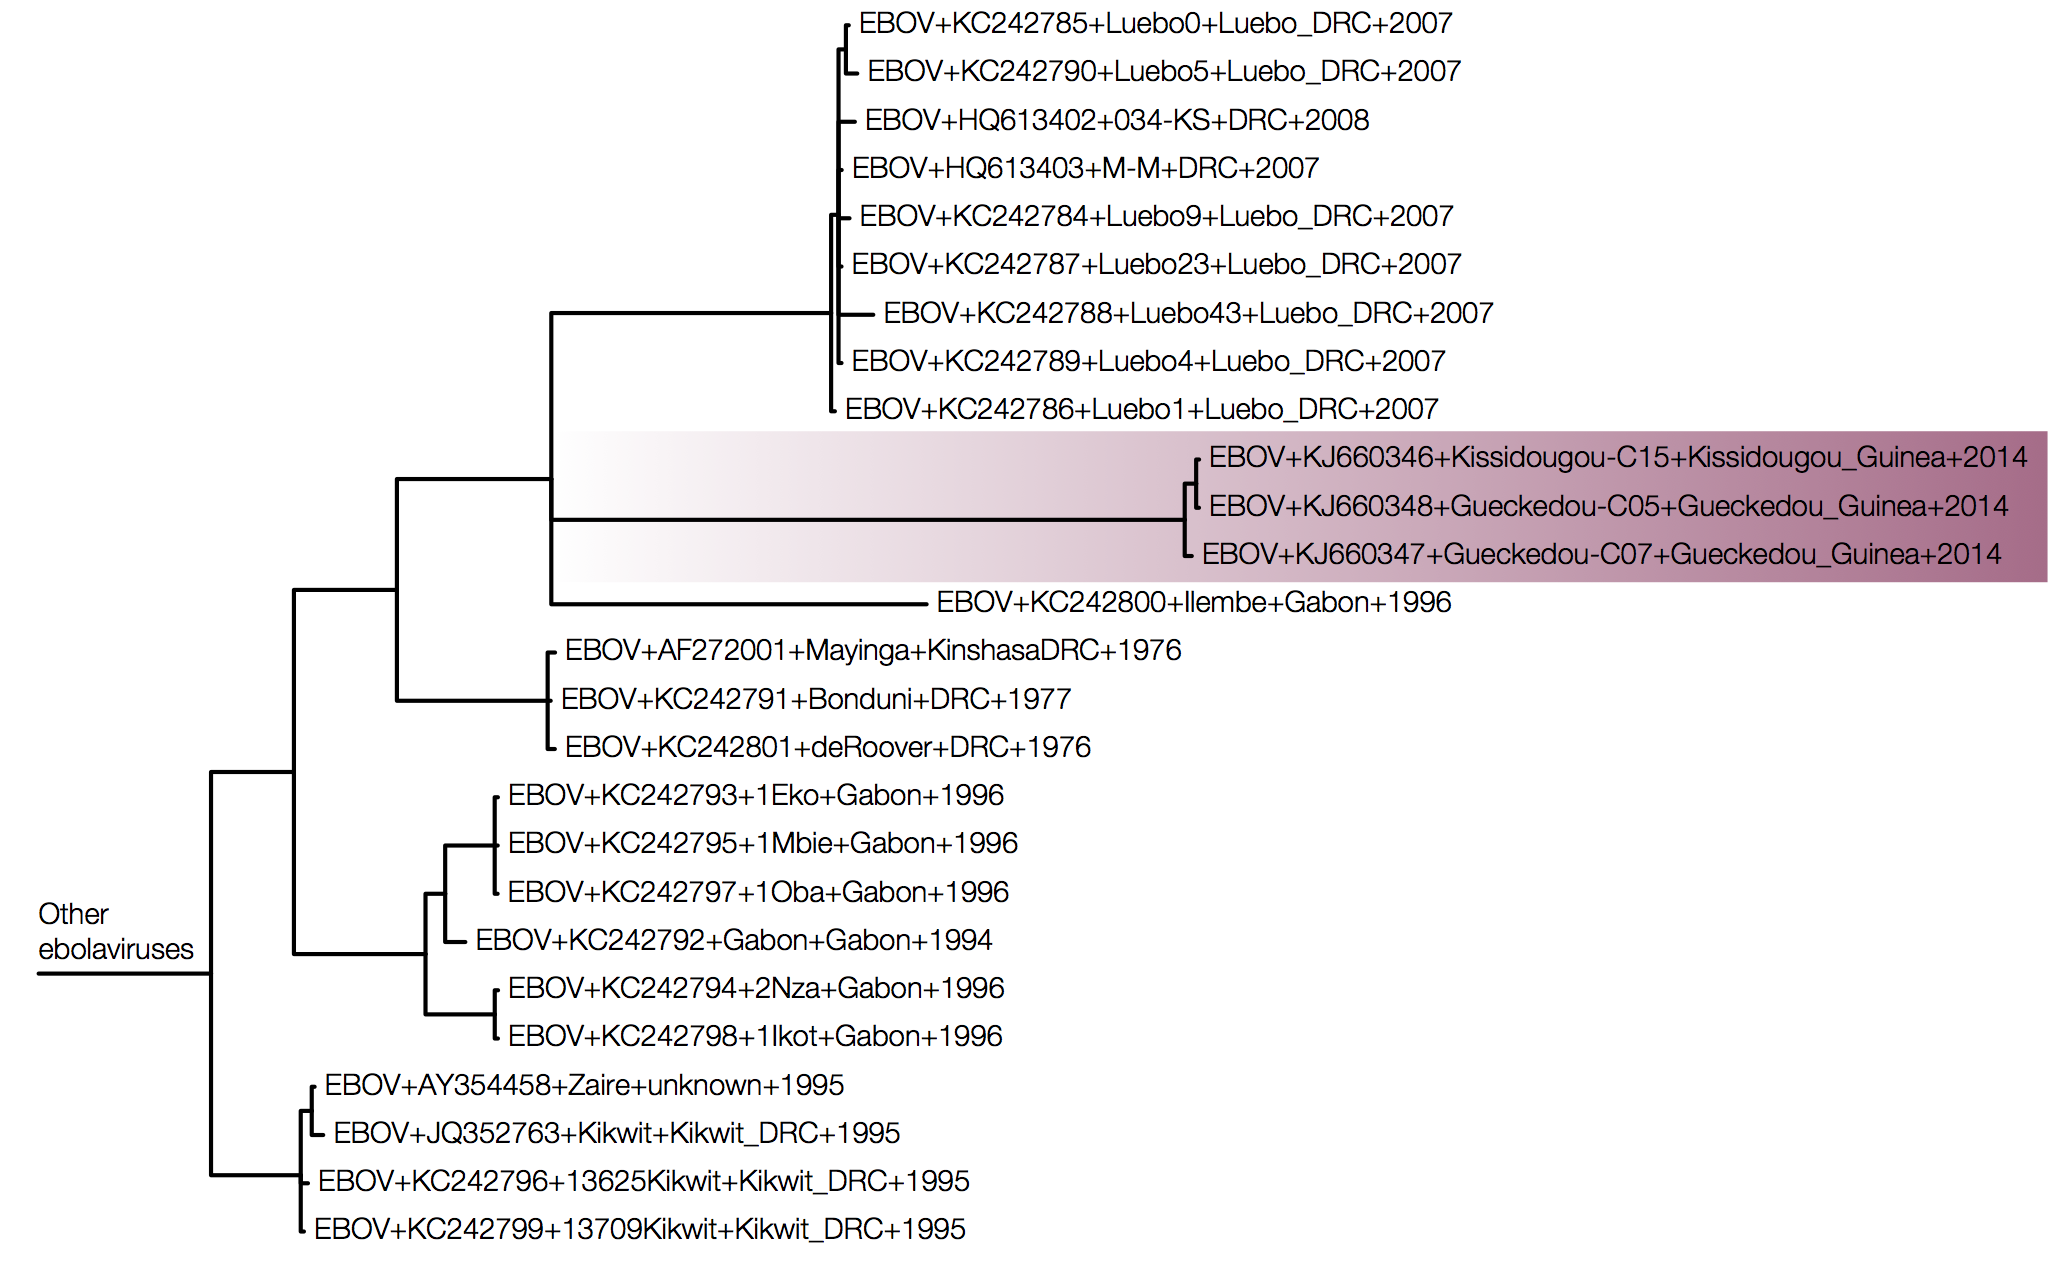
\includegraphics[width=0.9\textwidth]  {figures/EBOV_intergenic_mb_tree.png}
\caption{\textbf{MrBayes tree of intergenic sequences.}
Intergenic regions show a similar picture with the Guinea sequences nested within EBOV.}
\label{MBtreeIG}
\end{figure}

Figures \ref{MBtreeCDSzoomed} and \ref{MBtreeIG} show MrBayes trees from protein coding and intergenic regions of the EBOV genome, respectively, with more divergent ebolavirus strains cropped out.
Note that trees in Figures \ref{MBtreeCDSzoomed} and \ref{MBtreeIG} are essentially identical but differ by where the other ebolavirus species root the EBOV clade (on the 2007 Gabon outbreak for the coding regions in Figure \ref{MBtreeCDSzoomed} and on the 1995 Kikwit outbreak for the intergenic regions in Figure \ref{MBtreeIG}). This shows that the rooting of this clade using the very divergent other ebolavirus species is very problematic. 

However, EBOV is estimated to evolve at about $7\times10^{-4}$ substitutions per site per year \cite{carroll2013} which means that the virus will accumulate significant amounts of substitutions over the nearly 40 years since the first recorded outbreak in 1976.
We can use this to root the EBOV tree and look at where the Guinea outbreak lies.
Path-O-Gen (available at \url{http://tree.bio.ed.ac.uk/software/pathogen/}) was used to find the root that gave the best association between genetic divergence and time.
The relationship between genetic divergence and time after rooting the tree using least squares regression is shown in Figure \ref{MBPath}.

\begin{figure}[h!]
\centering  
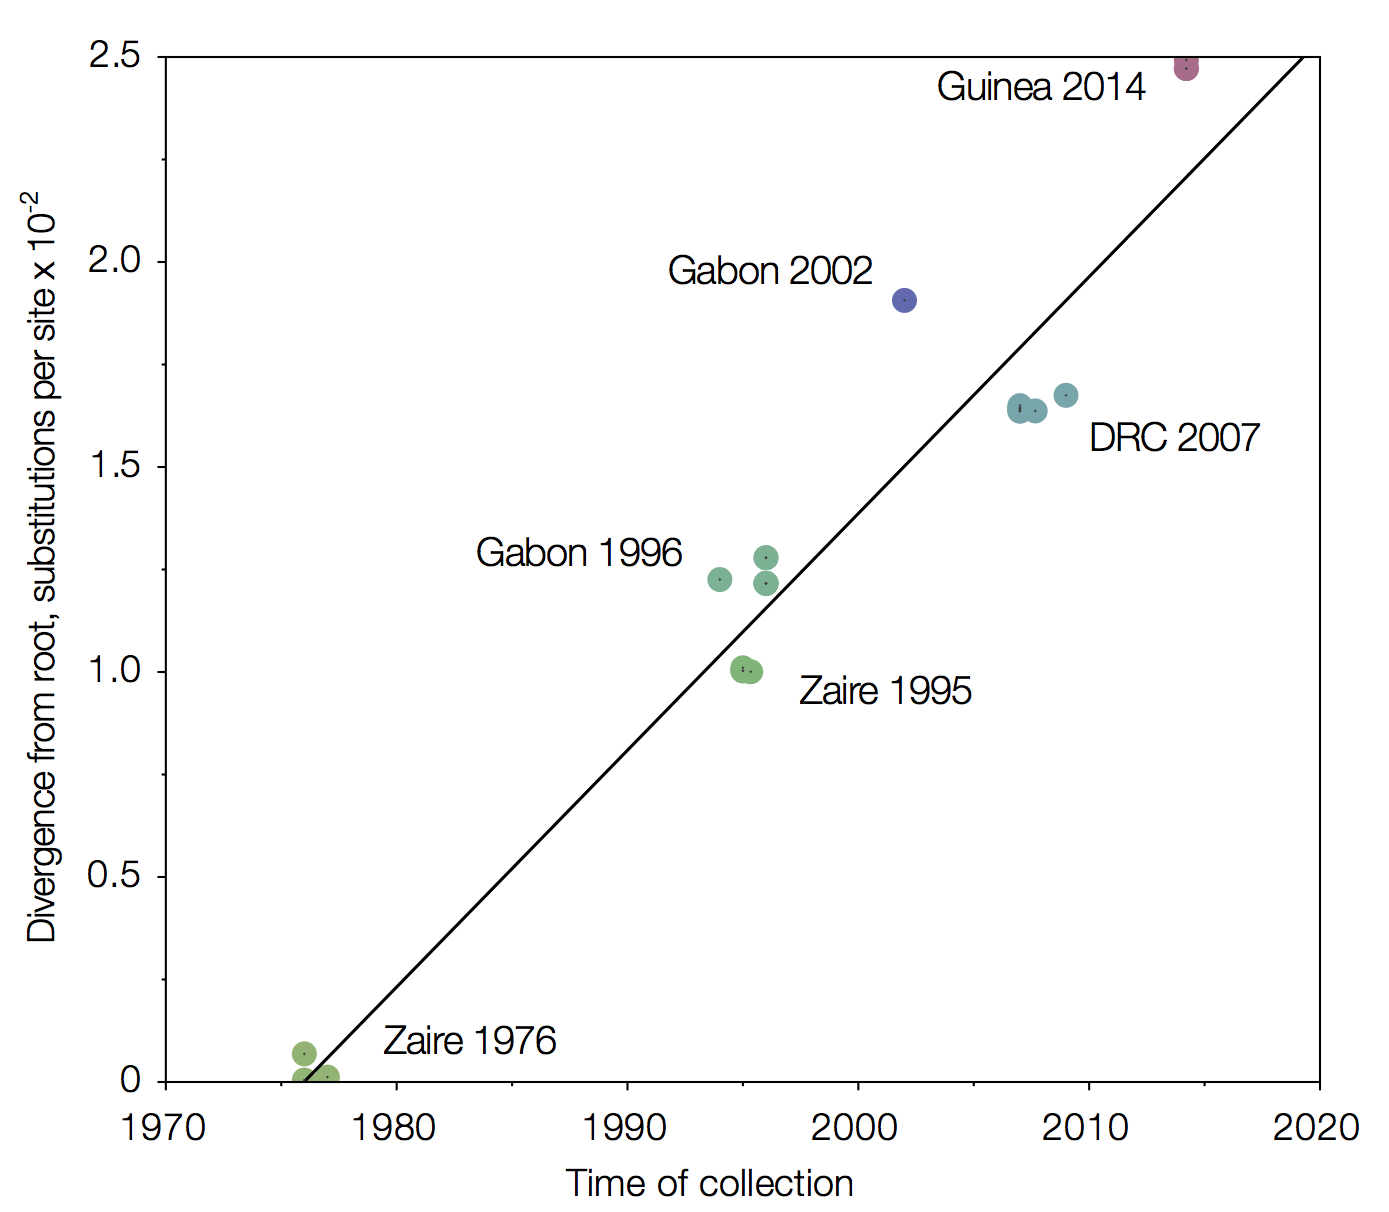
\includegraphics[width=0.6\textwidth]  {figures/EBOV_cds_mb_path.png}
\caption{\textbf{Root-to-tip regression of a MrBayes tree of concatenated coding regions.}
Sequences from the 1976 Zaire outbreak are very close to the root.}
\label{MBPath}
\end{figure}

Figure \ref{MBtreePath} shows the phylogeny of the coding sequences recovered by MrBayes (a maximum likelihood tree using PhyML gave an almost identical tree) rooted by least squares regression.
The root of this tree is very close to the earliest sequences from the 1976 Zaire outbreak.

\begin{figure}[h!]
\centering  
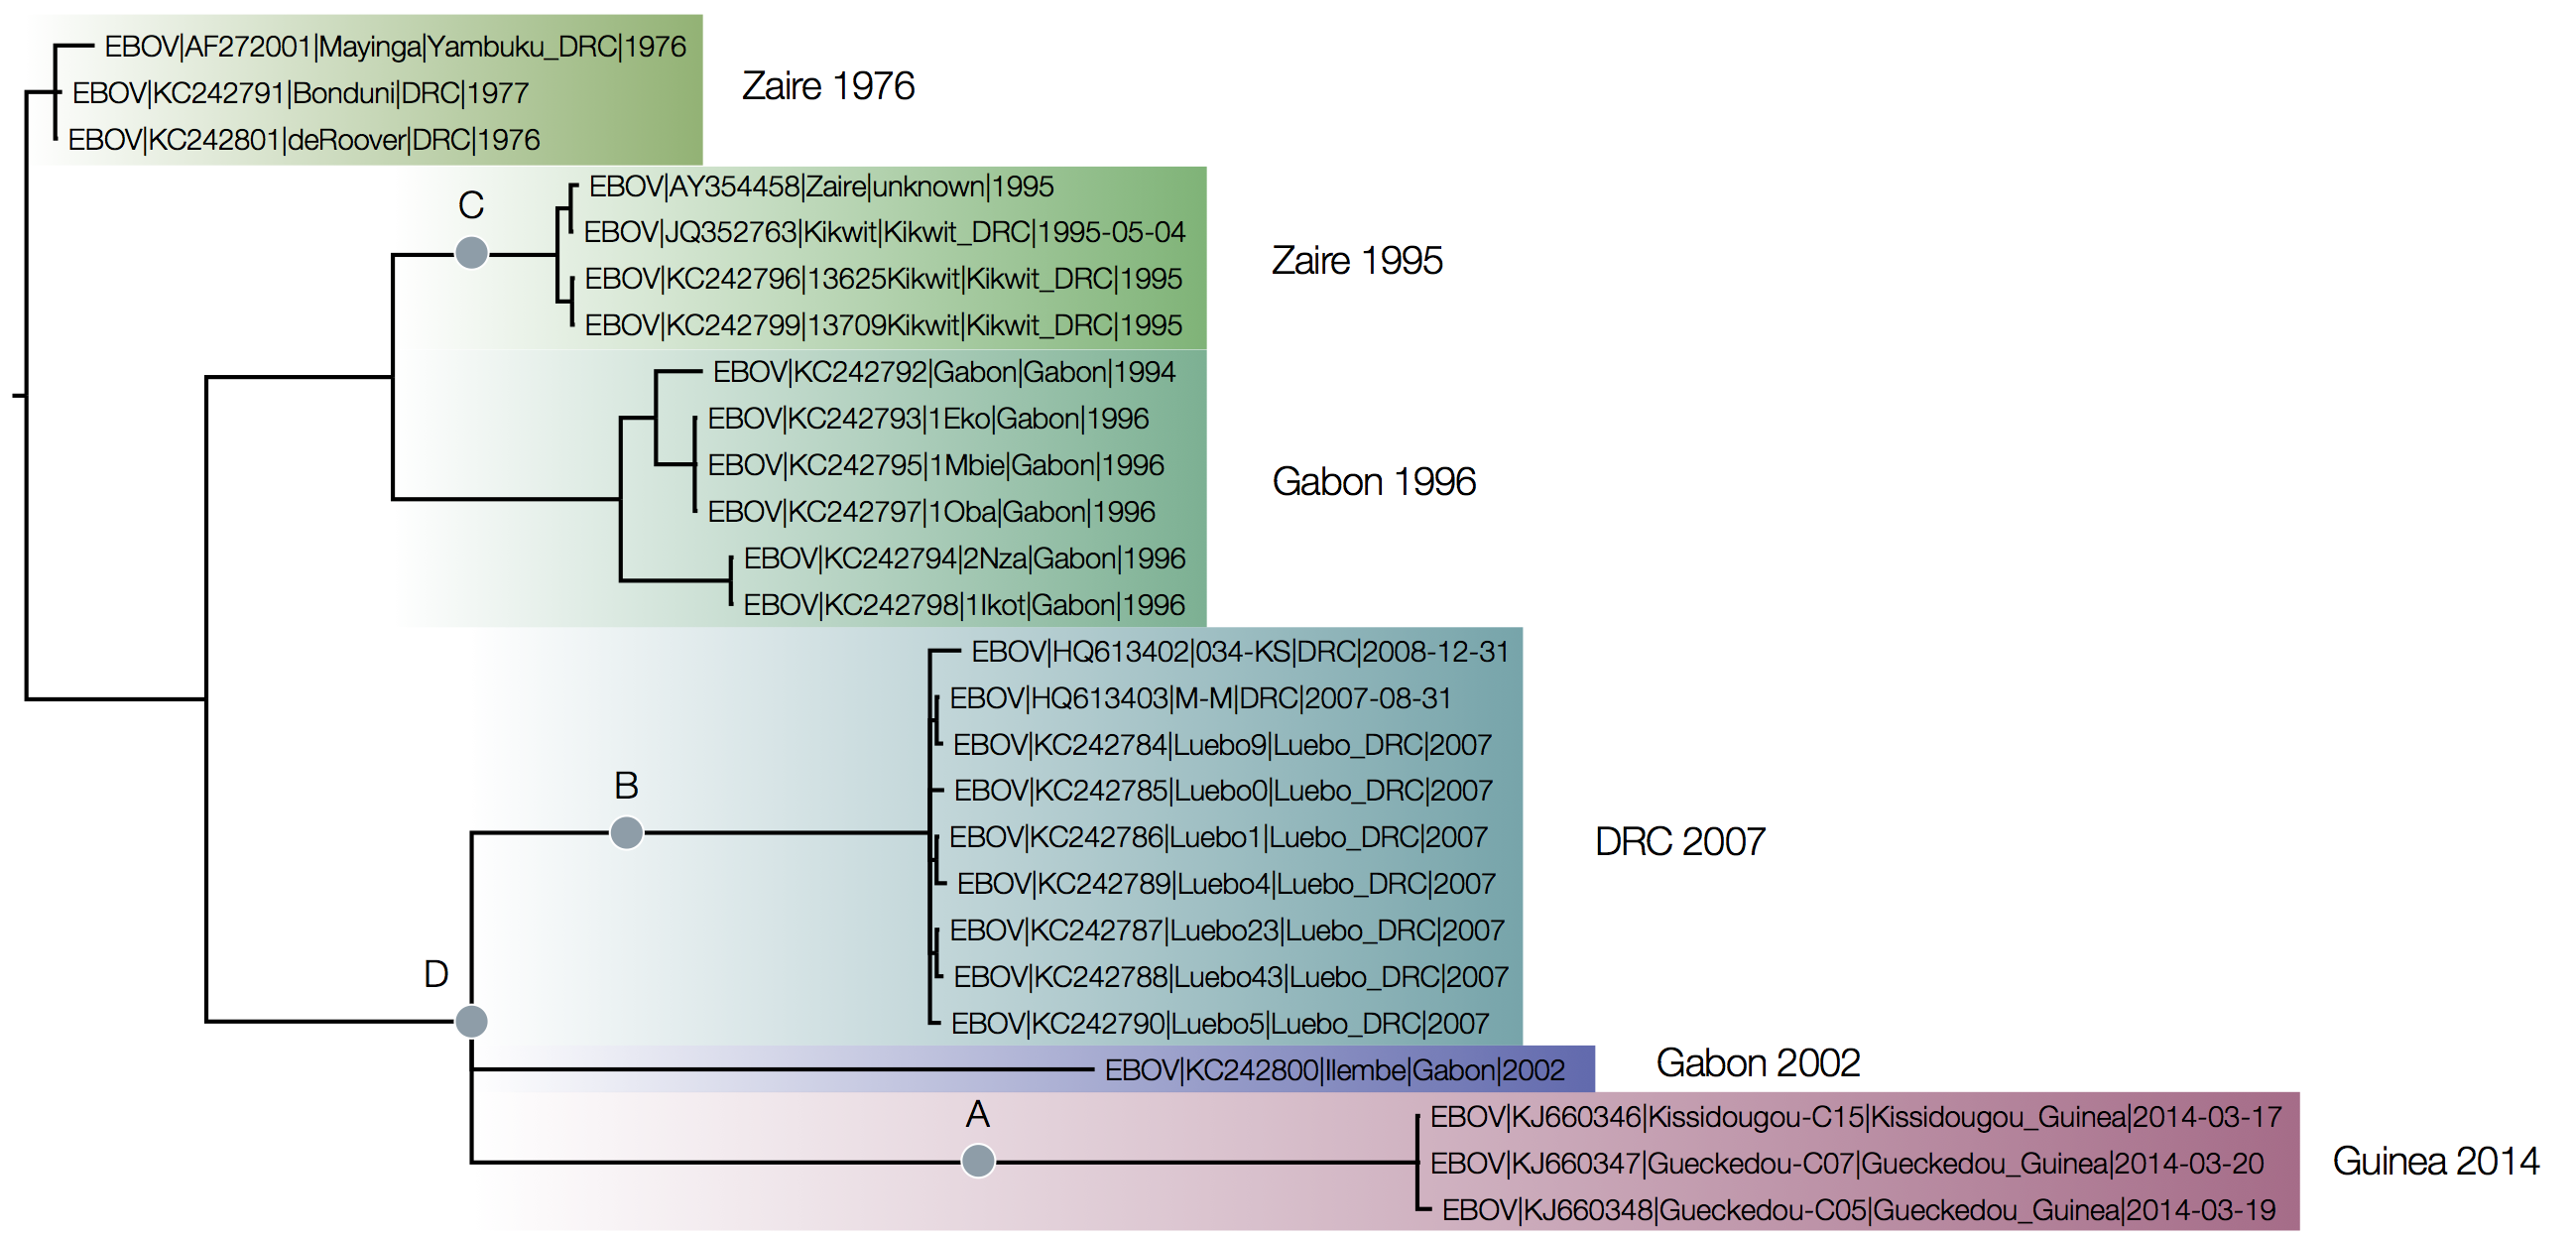
\includegraphics[width=0.9\textwidth]  {figures/EBOV_cds_mb_rootedTree.png}
\caption{\textbf{MrBayes tree of concatenated coding sequences rooted by least squares regression.}
The Bayesian posterior support for all the groupings between the outbreaks are 1.0 including for the grouping of Guinea 2014 with DRC 2007 and Gabon 2002. This demonstrates that the uncertainty about the position of the Guinea 2014 lineage in the complete ebolavirus trees was down to the rooting of the EBOV clade (\textit{i.e.}, where the divergent outgroups connect to the EBOV tree). The relationships of the EBOV outbreaks is completely consistent for the simple whole genome alignment, the coding regions only and the intergenic regions only but the position of the root changes. In the above figure, A) denotes the position of the root for the full genome maximum likelihood tree, B) for the Bayesian coding-sequence only tree, C) the Bayesian intergenic regions only tree and D) the combined coding-sequence and intergenic region accommodating different rates of evolution.}
\label{MBtreePath}
\end{figure}

\section*{Estimating the date of introduction of EBOV into Guinea}
The analysis of GP sequences in BEAST revealed rooting consistent with that found in Figure \ref{MBtreePath} as well as a nucleotide substitution rate (mean of lognormal distribution from which rates were drawn is $1.073\times10^{-3}$, 95\% HPD interval $5.9891\times10^{-4}$ -- $1.7494\times10^{-3}$) on a scale expected, given previously published rates \cite{carroll2013} and the fact that GP codes for a surface glycoprotein.
In Figure \ref{beastTree} the estimate of the split between the lineage now causing an outbreak in Guinea and the Central African lineage that had caused outbreaks in DRC and Gabon is around 2002 November (95\% HPD interval 2000 March -- 2006 February).
This gives us a lower boundary on the introduction of DRC/Gabon lineage of EBOV into Guinea, although these estimates should be interpreted with caution.
We also find very good support for the common ancestry of Guinea and DRC/Gabon lineages (posterior probability = 1.0).
Figure \ref{beastTree} also highlights the importance of environmental sampling - many sequences in the tree come from ape carcasses and are more diverse (not shown) than sequences from human outbreaks, giving this dataset much better resolution.

\begin{figure}[h!]
\centering  
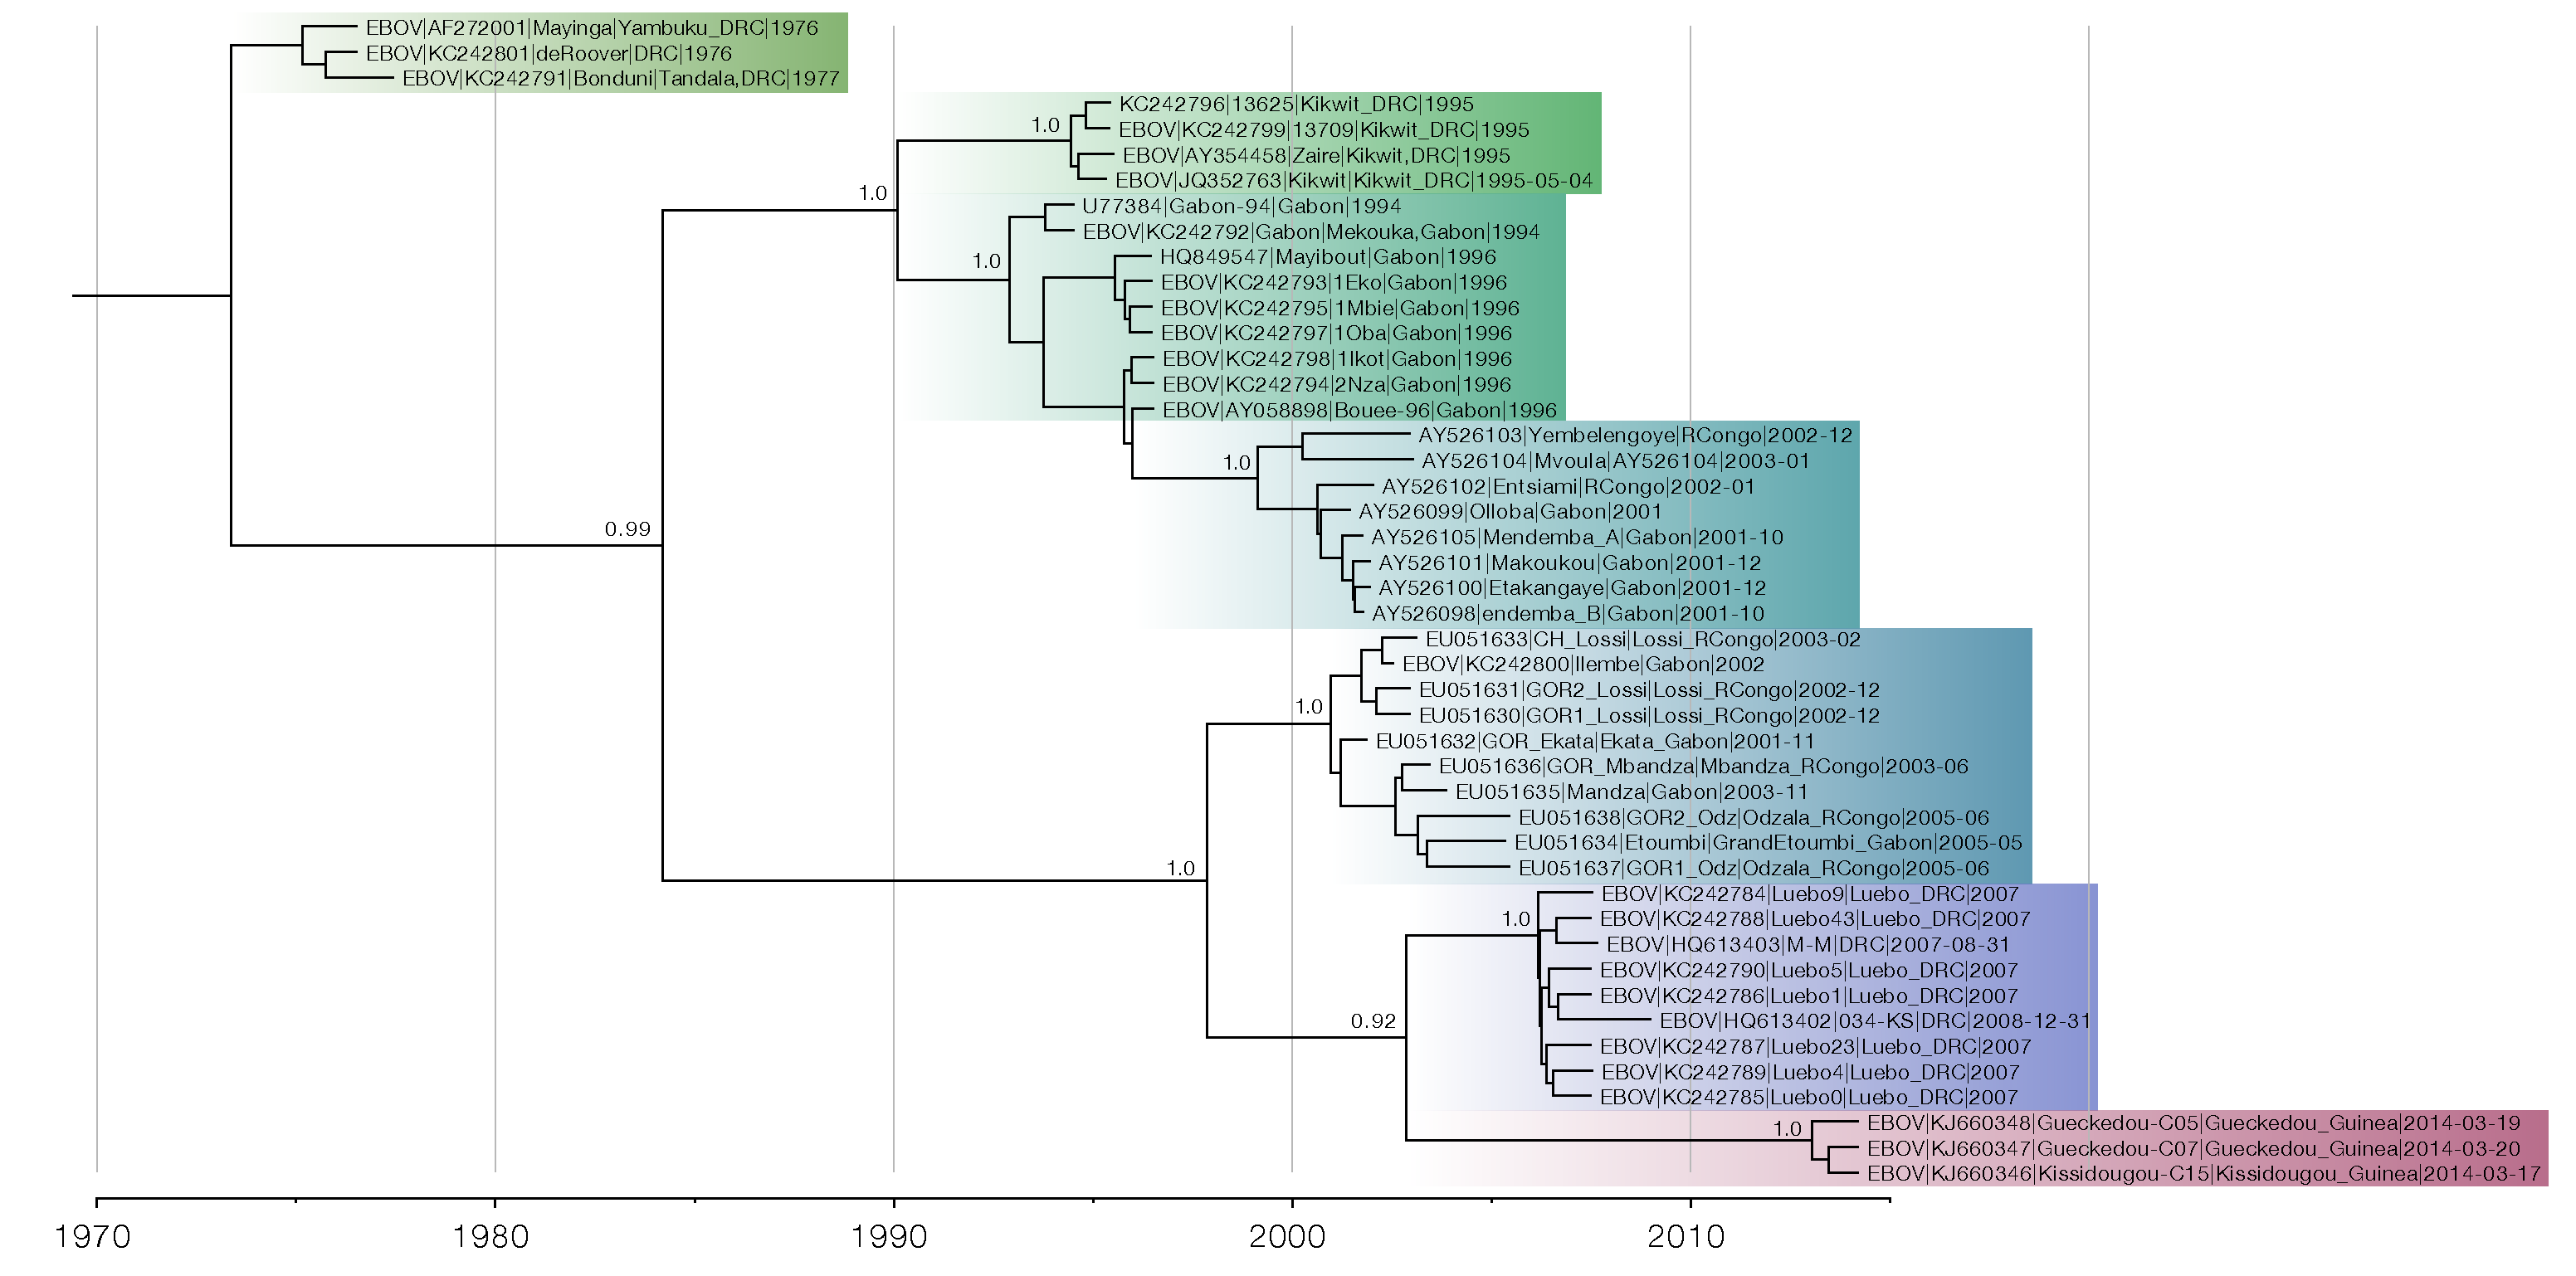
\includegraphics[width=1\textwidth]  {figures/EBOV_GP_46_GTRG_UCLN_EGC_MCC_tree.pdf}
\caption{\textbf{Maximum clade credibility tree of GP sequences.}
Although the closest relatives of the Guinea lineage are not entirely certain (posterior probability 0.92), its relationship with Central African EBOV lineages is well-supported (posterior probability 1.0).}
\label{beastTree}
\end{figure}

\section*{Conclusion}
Overall, our analyses only marginally improve upon those of Baize \textit{et al}. \cite{baize2014}, due to paucity of sequence data. 
We find that at this time no suitable outgroup sequences to root the EBOV phylogeny exist and that temporal rooting gives the most consistent results.
Our analyses also indicate that the outbreak in Guinea is likely caused by a Zaire ebolavirus lineage that has spread from Central Africa into Guinea and West Africa, not a divergent endemic lineage.
As the GP sequences show, without more diverse sequences, especially those from the animal reservoir, it is difficult to narrow down the estimates of when and through what means the Central African EBOV lineage has been introduced into West Africa.

\section*{Acknowledgements}
GD was supported by a NERC studentship D76739X.
The research leading to these results has received funding from the European Research Council under the European Community's Seventh Framework Programme (FP7/2007-2013) under Grant Agreement no. 278433-PREDEMICS and ERC Grant agreement no. 260864.
AR acknowledges the support of the Wellcome Trust (grant no. 092807).

\bibliographystyle{plos}
\bibliography{ebolaGuinea2014}

\end{document}